\section{V3 Uncertainty Framework}

Figure~\ref{fig:v3-pipeline} summarizes the v3 evidence flow. The starting point remains the calibrated proxy-surface identity inherited from v2. V3 then adds an ensemble layer, interval summaries, bounded confidence bands, hotspot prioritization, and a validation package designed to test whether the uncertainty layer behaves meaningfully inside the proxy framework.

\begin{figure}[H]
\centering
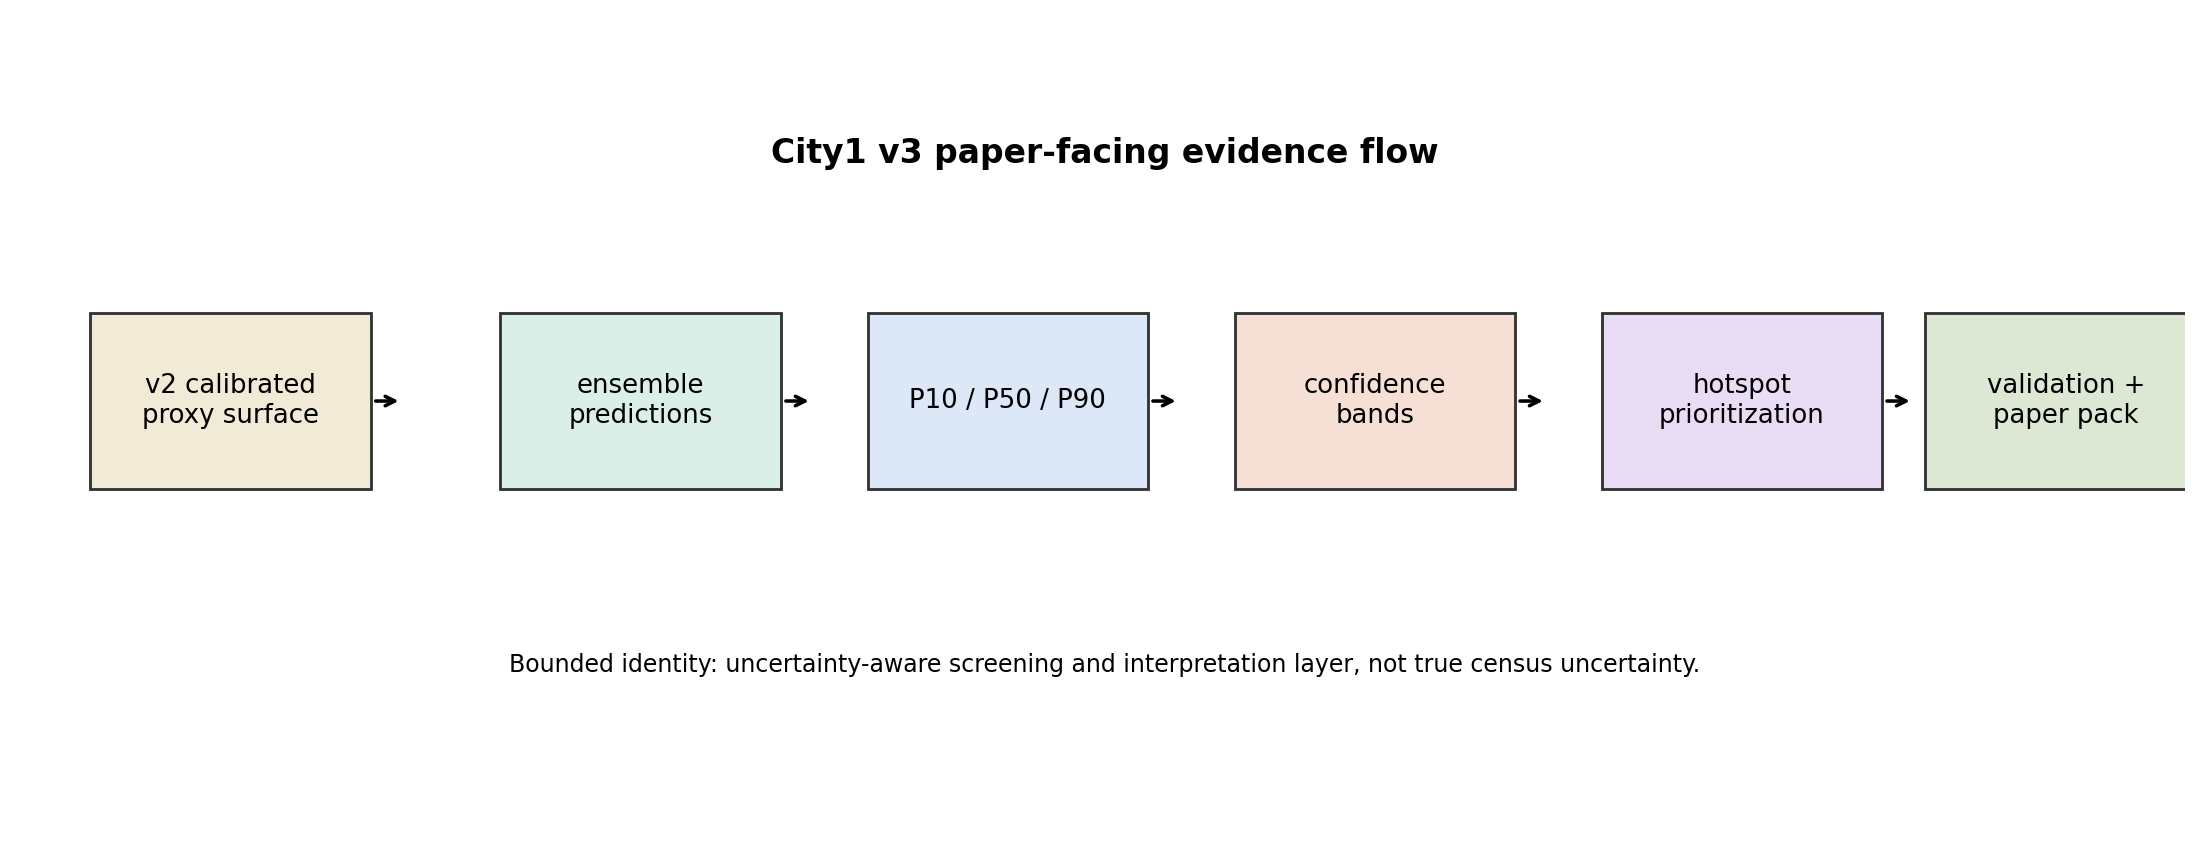
\includegraphics[width=\textwidth]{figures/fig1_v3_pipeline.png}
\caption{City1 v3 paper-facing evidence flow. The deterministic calibrated proxy surface is extended through ensemble predictions, empirical proxy intervals, confidence bands, hotspot prioritization, and a validation/paper package. This figure shows the v3 interpretation stack; it does not imply true census-uncertainty estimation.}
\label{fig:v3-pipeline}
\end{figure}

\subsection{Frozen run configuration}

The full frozen v3 run is identified by \texttt{city1\_v3\_rf500m\_e20\_20260618T040646Z}. The core training artifact uses a random-forest ensemble with 20 members, a fixed 500 m grid, within-city bootstrap resampling, log-target training, and the same 17 frozen feature columns carried from the v2 baseline. The training package reports 8 training cities and 16,132 training rows. The frozen inference set used for the paper-facing package contains four cities: Almaty, Astana, Semey, and Shymkent.

\subsection{Calibrated ensemble members and interval outputs}

Let $\hat{y}^{(m)}_{i,c}$ denote the raw prediction for cell $i$ in city $c$ from ensemble member $m$, and let $P_c$ denote the official city total. Each ensemble member is calibrated separately:
\[
\hat{y}^{(m),\mathrm{cal}}_{i,c}=
\hat{y}^{(m)}_{i,c}\cdot
\frac{P_c}{\sum_{j \in c}\hat{y}^{(m)}_{j,c}},
\]
whenever the within-city raw sum is positive. If that sum is non-positive, the workflow falls back to a uniform within-city allocation so that calibration remains well defined. The calibrated member ensemble is then summarized per cell through empirical quantiles:
\[
\mathrm{P10}_i = Q_{0.10}\!\left(\hat{y}^{(m),\mathrm{cal}}_{i,c}\right), \qquad
\mathrm{P50}_i = Q_{0.50}\!\left(\hat{y}^{(m),\mathrm{cal}}_{i,c}\right), \qquad
\mathrm{P90}_i = Q_{0.90}\!\left(\hat{y}^{(m),\mathrm{cal}}_{i,c}\right).
\]

The median surface, $\mathrm{P50}$, is retained as the canonical final v3 proxy surface and is stored as the backward-compatible alias \texttt{Population\_Estimate\_Final}. Interval width and relative uncertainty are defined as:
\[
\mathrm{width}_i = \mathrm{P90}_i - \mathrm{P10}_i,
\qquad
r_i = \frac{\mathrm{width}_i}{\max(\mathrm{P50}_i,\epsilon)},
\]
where $\epsilon$ is a small positive constant from the frozen configuration.

\subsection{Confidence scores and bands}

City1 v3 does not treat uncertainty as a probability of correctness. Instead, it defines a bounded interpretation-confidence score. The first component is a model-stability term based on city-relative uncertainty burden:
\[
s_i = 1 - \operatorname{clip}\!\left(
\frac{r_i}{\max(q_{0.90}^{(c)},\epsilon)}, 0, 1
\right),
\]
where $q_{0.90}^{(c)}$ is the 90th percentile of relative uncertainty in city $c$. This stability term is then combined with frozen city-level support components for OSM completeness, external benchmark context, and internal district-support context:
\[
\mathrm{confidence}_i =
\operatorname{clip}\!\left(
0.40\,s_i +
0.25\,o_c +
0.20\,e_i +
0.15\,d_c, 0, 1
\right).
\]
Here $o_c$ is the normalized OSM support score, $e_i$ is the best available external-agreement support component or neutral fallback, and $d_c$ is the internal-support component or neutral fallback. The exact formula and component definitions are restated in Supplementary Section~S2.

Confidence bands are then assigned through fixed thresholds: high for scores at least 0.70, medium for scores in $[0.40,0.70)$, and low for scores below 0.40. These bands are meant to structure interpretation. They are not posterior probabilities and must not be read as truth guarantees.

\subsection{Hotspot prioritization classes}

The practical v3 use case is uncertainty-aware hotspot prioritization. Cells are ranked within each city by calibrated median surface value. High-value cells are defined by the city-specific top decile of $\mathrm{P50}$. The frozen class vocabulary distinguishes stable screening candidates from caution-heavy ones:

\begin{itemize}
\item \texttt{high\_value\_high\_confidence},
\item \texttt{high\_value\_low\_confidence},
\item \texttt{medium\_value\_high\_confidence},
\item \texttt{low\_value\_high\_uncertainty},
\item \texttt{not\_priority}.
\end{itemize}

These classes are useful because they transform the uncertainty layer into an interpretable screening output. They do not prove that a hotspot is a true population center, nor that a low-confidence hotspot is wrong. They indicate which parts of the proxy surface are more stable candidates for exploratory prioritization and which parts should be treated as review-oriented.

\subsection{Bounded validation setting}

The paper-facing uncertainty evidence is linked to the same frozen run, but one part of Phase 6 used a bounded local reconstruction setting for cost control: a LOCO-like validation pass with 5 ensemble members and 60 trees per member. This limitation is carried forward explicitly in the manuscript and the supplement. The full inference package remains the 20-member frozen run.

